\documentclass[tikz]{standalone}
\usetikzlibrary{calc}

\definecolor{blue}{HTML}{1F78B4}
\definecolor{red}{HTML}{E31A1C}
\definecolor{grey80}{HTML}{CCCCCC}

\begin{document}
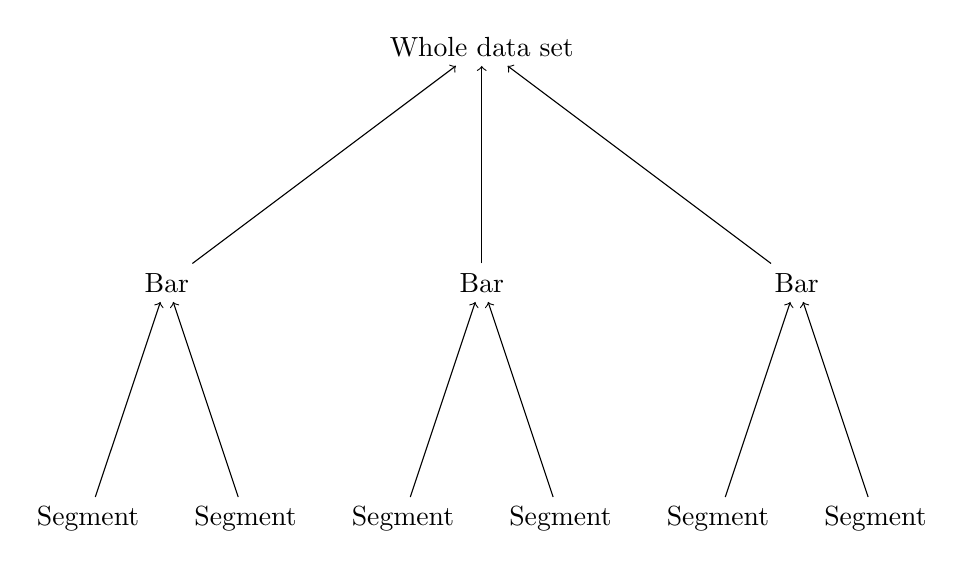
\begin{tikzpicture}[scale=1.0]

  \node (data) at (7, 6) {Whole data set};
  \node (bar1) at (3, 3) {Bar};
  \node (bar2) at (7, 3) {Bar};
  \node (bar3) at (11, 3) {Bar};
  \node (seg1) at (2, 0) {Segment};
  \node (seg2) at (4, 0) {Segment};
  \node (seg3) at (6, 0) {Segment};
  \node (seg4) at (8, 0) {Segment};
  \node (seg5) at (10, 0) {Segment};
  \node (seg6) at (12, 0) {Segment};

  \draw (bar1) edge[->] (data);
  \draw (bar2) edge[->] (data);
  \draw (bar3) edge[->] (data);

  \draw (seg1) edge[->] (bar1);
  \draw (seg2) edge[->] (bar1);
  \draw (seg3) edge[->] (bar2);
  \draw (seg4) edge[->] (bar2);
  \draw (seg5) edge[->] (bar3);
  \draw (seg6) edge[->] (bar3);

\end{tikzpicture}
\end{document}
